% !TEX root = main.tex
\section{Exposure reverses the ranking}
\label{sec:ranking}

\subsection{A large exposure effect that misses retention}
\label{sec:exp01}
% Provenance: experiments/archive/01_fixed_width_addition_exposure/RESULTS_addition_exposure.md
In \texttt{experiments/archive/01\_fixed\_width\_addition\_exposure/}, one 29{,}480-parameter network is trained from scratch for 3{,}000 updates on 16{,}000 pairs.
The fixed test set has 1{,}000 pairs in each carry-chain length, evaluated under eight seeds (8{,}000 predictions per cell, not 8{,}000 independent items).
With 97\% no-carry training, no-carry accuracy is 100.00\% [100.00, 100.00] and length-three-carry accuracy is 9.60\% [7.85, 11.22].
With 97\% length-three-carry training, those same groups score 6.84\% [5.79, 7.79] and 100.00\% [100.00, 100.00].
Balanced training moves length-three accuracy from 9.60\% to 94.89\% (7{,}591/8{,}000) and recovers 94.34\% [92.74, 95.86] of the 90.40-point baseline gap.
The prospective retention rule allows no-carry accuracy to fall by at most 5 points.
It falls from 100.00\% to 93.92\%, a change of $-6.08$ [$-8.39$, $-4.11$] percentage points.
Five of six frozen criteria pass, and the aggregate verdict is not established.
An auxiliary sign-flip test of the length-three gain against half the baseline gap gives p-val=$0.00390625$ under an exhaustive paired sign enumeration.
That test does not override the failed retention criterion.
The shuffled-label control scores 22/32{,}000 exact sums (0.06875\%), below the protocol's 5\% ceiling.
Balanced training also makes length-one chains less accurate than length-three chains (73.92\% versus 94.89\%).
Carry-chain length is therefore not an empirically monotone difficulty scale in this run.
The extreme mixtures also change digit and answer frequencies, so the contrast is the whole distribution intervention.

\subsection{Answer matching preserves the reversal}
\label{sec:exp03}
% Provenance: experiments/archive/03_answer_matched_alignment/RESULTS_matched_alignment.md
\texttt{experiments/archive/03\_answer\_matched\_alignment/} gives every intervention exactly 40 training pairs for each of 117 sums (4{,}680 pairs).
The two evaluation strata have identical answer histograms, with 936 fixed items each.
After 500 shared balanced warmup updates, a 90\% no-carry intervention favors no-carry items by 25.30 [23.14, 27.26] percentage points at 3{,}000 updates.
A 90\% two-carry intervention favors two-carry items by 24.58 [22.88, 26.19] points.
Seed standard deviations of those two contrasts are 3.21 and 2.56 points.
Both lower endpoints are positive, and both contrasts are positive at each of the five widths.
The frozen ranking gate is supported.
The lead shrinks with width: 66.16 and 67.49 points at width 32, and 2.30 and 1.46 points at width 256.
The gate requires a pooled lead of at least 10 points and a positive point at every width.
It does not require a 10-point lead at every width.
Figure~\ref{fig:alignment} shows the reversal.
Input-digit total variation between the endpoint mixtures remains large, from 0.0668 to 0.6469 across the six digit positions.
Answer matching does not isolate carrying from the input digits.

\begin{figure}[t]
\centering
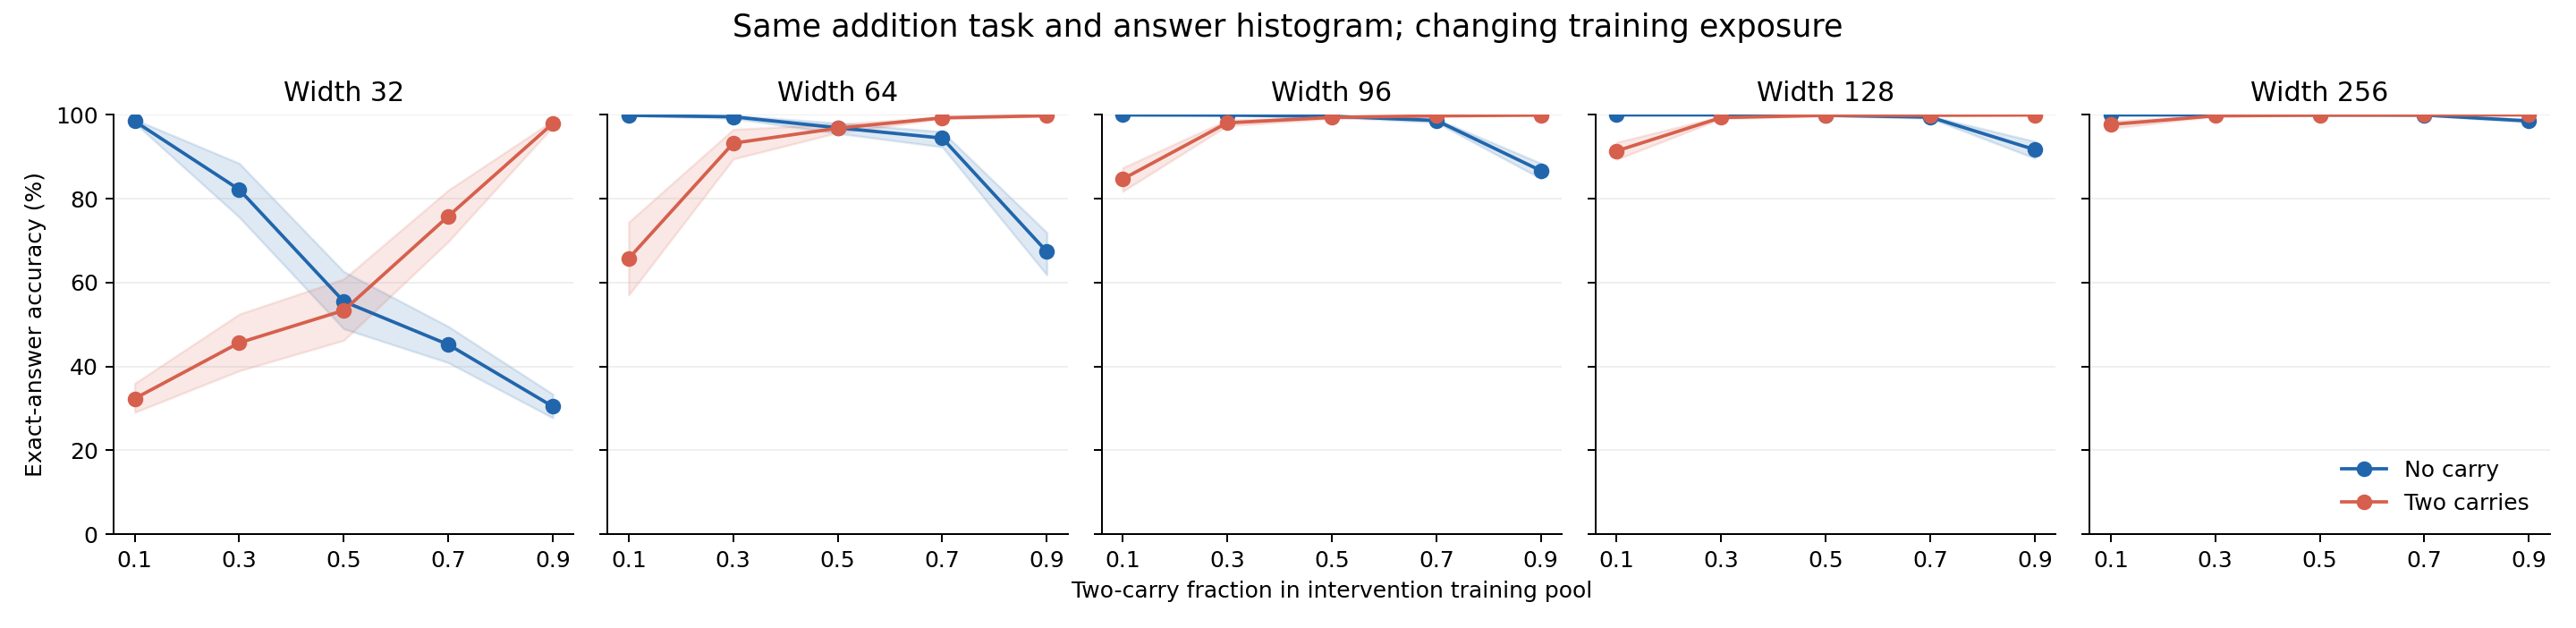
\includegraphics[width=\linewidth]{../../experiments/archive/03_answer_matched_alignment/expt_v1/results/alignment_accuracy.png}
\caption{\textbf{Answer-matched exposure reverses which stratum is more accurate.} Accuracy of no-carry and two-carry items against the two-carry training fraction, for \texttt{experiments/archive/03\_answer\_matched\_alignment/}.
Shading in the source figure is the paired-seed interval.
Eight seeds, 936 fixed items per stratum, p-val=n/a.
The same items change rank as the mixture changes.}
\label{fig:alignment}
\end{figure}

\subsection{The reversal survives matched carry rates}
\label{sec:exp06}
% Provenance: experiments/archive/06_compositional_carry_marginal_matched/RESULTS_compositional.md
% and expt_v1/results/prediction_comparisons.csv for the repair row.
\texttt{experiments/archive/04\_monotone\_ridge\_heldout\_addition/} repeats the answer-matched reversal on fresh items, seeds, and widths.
The endpoint leads are 24.07 [22.80, 25.46] and 24.48 [22.77, 26.06] percentage points, and the ranking gate is supported.
At width 384 the leads are 0.55 and 0.24 points, still positive and far below the pooled 10-point bar.
\texttt{experiments/archive/06\_compositional\_carry\_marginal\_matched/} then matches both the answer histogram and the per-column carry rates.
Every mixture has exactly 3{,}600/7{,}200 ones-column carries and 3{,}600/7{,}200 tens-column carries.
Endpoint input-digit total variation falls from a mean of 0.443 (maximum 0.656) in the previous answer-matched studies to a mean of 0.0398 (range 0.0049 to 0.0972).
The contrast is between isolated single carries, ones-only or tens-only, and a cascading two-carry cell.
At a 10\% compositional mixture, single carries lead by 22.35 [20.60, 24.00] points.
The two single-carry cells score 93.62\% [91.51, 95.60] and 93.78\% [91.93, 95.55], against 71.35\% [69.31, 73.66] on the two-carry cell.
At a 90\% compositional mixture, the two-carry cell leads by 17.74 [14.62, 21.12] points.
That cell scores 92.13\% [90.07, 94.07], against 74.28\% [70.55, 77.38] and 74.49\% [71.23, 77.84] on the single-carry cells.
Both directions are positive at all five widths, and the ranking gate is supported.
The residual structure contrast is 2.30 [1.02, 3.51] points, much smaller than the 20.05 [17.75, 22.32] alignment contrast.
Matching the column rates does not remove the reversal.
It also does not make the reversal the same size at every width: width 384 leads by 7.04 and 3.01 points.
